\section{Requirements and concept}

\subsection{Challenges and requirements in Audio Signal Processing}

\subsubsection{Latency}

As we have to sample a block of data in the digital domain, there is a latency between the input and output
depending on some parameters. Firstly the buffer size has a large impact on the latency. The greater the buffer the
greater the latency. It is application depending what latency is acceptable, this is why that parameter
limits the system and should be evaluated carefully.

Secondly other components, which are application depending, adds latency to the whole signal path.
For example filtering or other modifications take some time to be computed. Also the signal has to
be converted from analog to digital and transmitted over an interface. All these components latencies add
up to an overall system latency. 

In this application, where a guitar signal is processed, the overall latency of the system should be less
than 5\,ms \cite{beckmann_dsp}. %// TODO: evaluate!

\subsubsection{Packet losses and cracking noise} %// TODO: buffer size evaluate?

In some audio applications cracking noise can occur. This is due to
some impulses on the audio signal. This can be caused by an error of the input sample, for example particles
on a vinyl record, or by slow implementations of digital signal processing algorithms.

If the processing of the input data takes longer than the actual transfer, packets of audio data will
then be dropped. An impulse or step on the output data will be seen, this can be heard as a cracking noise
\cite{stotz_audio_video}.

\subsection{Concept}

The basic concept is shown in \autoref{fig:basic-concept}.

\begin{figure}[!h]
    \centering
    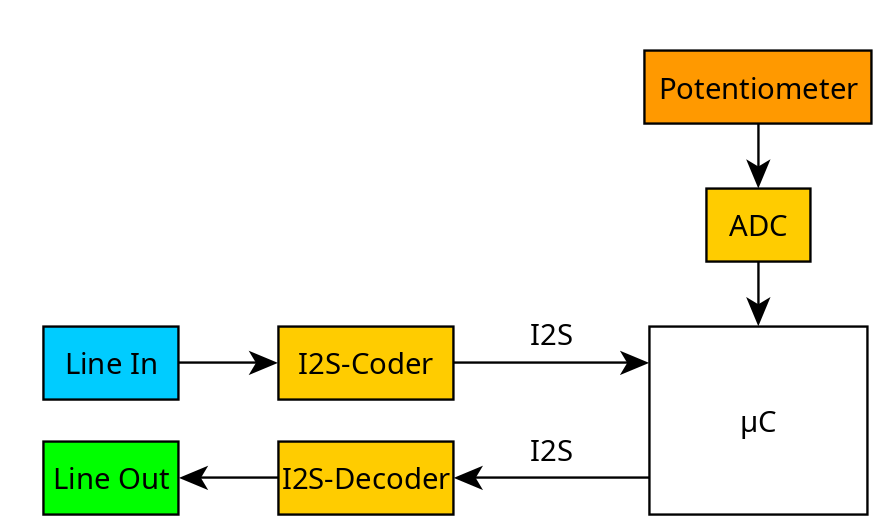
\includegraphics[width=7cm]{img/basic_concept.PNG}
    \caption{Basic concept}
    \label{fig:basic-concept}
\end{figure}

The input data is coming from the Line In, is sampled by a \ac{ADC} and transmitted
over \ac{I2S} to the microcontroller. There the data will be processed and the output will be transmitted
again over \ac{I2S} to a \ac{DAC}. The output is again routed to a Line Jack.

Additionally a potentiometer is connected to set the midfrequency of the filter.

There is also a serial connection to a PC where a \ac{CLI} should be available to configure
different parameters.

\subsubsection{Signalflow}

The basic idea is to filter the input signal with a bandpass filter. The mid frequency should be derived
from a potentiometer which is simply connected to an \ac{ADC} inside the microcontroller. It has to be evaluated
how exaclty the filter is adjusted.

The first attempt will be a lookup-table and everytime the position of the
potentiometer changes, the corresponding filter coefficients will be loaded.

The second approach is, to calculate the filter coefficients for a biquad-filter if the value of the potentiometer changes.
This is reasonable to evaluate as the number of coefficients is small in comparison to a \ac{FIR}-filter.

\subsubsection{Double Buffering and DMA}

To solve the problem with packet losses it is recommended to use the double buffering method.
It is basically a buffer which is cut in half. If the first half is filled with data then this half
will be processed while the other half is filled with the second half of the input data. Is the second
half filled then this half will be processed and so on.

The advantage is that it is not necessary to wait for the whole input data block to process.
This will reduce the time between processing and sampling data \cite{eetimes_fund_dsp}.

To take advantage of this, it is useful to combine this technique with a \ac{DMA},
which is already discussed in section \ref{sec:dma}.

The whole procedure is shown in \autoref{fig:double-buffering}.

\begin{figure}[!h]
    \centering
    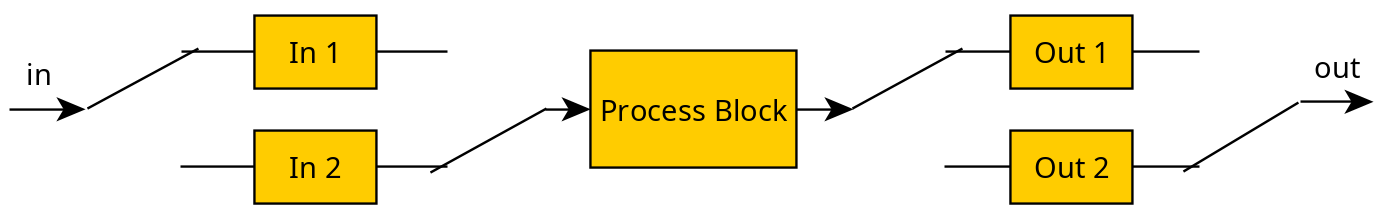
\includegraphics[width=11cm]{img/double_buffering.PNG}
    \caption{Double buffering concept \cite{eetimes_fund_dsp}}
    \label{fig:double-buffering}
\end{figure}
